% A TikZ picture inside another: a \tikz in a node's text, and the picture
% pgfplots' axis opens inside the user's. Each inner picture was captured on
% its own and left an empty placeholder in the outer one: its drawing and
% labels were lost, and a pgfplots axis came out blank.
\documentclass{article}
\usepackage{pgfplots}
\pgfplotsset{compat=1.18}
\begin{document}
A paragraph before the pictures, long enough to break across lines
differently at every width the test tries, so that each picture below
moves when the text is reflowed.

\begin{center}
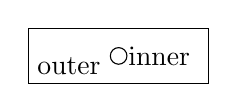
\begin{tikzpicture}
  \node[draw] at (0,0) {outer \tikz \draw (0,0) circle (3pt) node[right] {inner};};
\end{tikzpicture}
\end{center}
Text between the two pictures, with a few more words to fill the line.

\begin{center}
\begin{tikzpicture}
  \begin{axis}[width=6cm, xlabel={time $t$}, ylabel={value $v$}, title={A plot}]
    \addplot[domain=0:1] {x^2};
  \end{axis}
\end{tikzpicture}
\end{center}
A last paragraph after the plot.
\end{document}
